



\begin{frame}{\citetitle{MarcoNuno_Revista_2018_08_00} \footnotemark (1)}
\begin{block}{Problem description} 
 
		\begin{itemize}
		\item Teaching robotics is a challenge in many universities.   
\note[item]{\scriptsize The mathematics, electronics, electrical, control and mechanical concepts used in this area are hard to learn. Tools that facilitates the learning of this concepts are required}		
		\item A new technology for education is augmented reality (AR), that allows the co-existence of real and virtual objects in the same environment.  
\note[item]{\scriptsize In recent years, augmented reality has improved learning in several engineering areas}		
		\item AR can be combined with other techniques to enrich the applications, to
improve the teaching-learning process inside classrooms and laboratories.  
\note[item]{\scriptsize Areas that can be improved with AR are learning or robotics }
\item We propose a platform for teaching robotic arm manipulation concepts, having the following components: a homemade robotic arm, a control system, a desktop App and a Mobile App.   
\note[item]{\scriptsize  The home made robotic receives commands from the desktop app, moves each robotic arm articulation based on these commands. }
\item The mobile app uses AR to show the angles of the robotic arm articulations.  
\note[item]{\scriptsize The app allow the students to visualize in real time the response of the arm to the commands using AR.}
		\end{itemize}
\end{block} 
\footnotetext[1]{\fullcite{MarcoNuno_Revista_2018_08_00}}
\setcounter{footnote}{0}    
\end{frame}

\begin{frame}{\citetitle{MarcoNuno_Revista_2018_08_00} (2)}
\begin{block}{Proposed system} 
\begin{columns}
\begin{column}{0.5\textwidth}
\begin{enumerate}
\item The desktop application sends commands to the robotic arm control.  
\note[item]{\scriptsize Using a USB serial protocol.}
\item The robotic arm control moves the arm and sends back the angles of each articulation.  
%\note[item]{\scriptsize The robotic control generates the movement commands for each articulation, based on the information obtained from the desktop application.}
\item The mobile application sends a connection request to the robotic arm.   
\note[item]{\scriptsize The app uses a Bluetooth connection. } 
\item The mobile application identifies the markers located in the robot arm.  
%\note[item]{\scriptsize Once the connection is established, the mobile application identifies the markers located in the robot arm and sends a request to the robotic arm controller.}
\note[item]{\scriptsize Each robot articulation has a marker. In this specific case, we used only two markers, but this design can be extended to robotic arms with more than two articulations. }

\end{enumerate}
\end{column}
\begin{column}{0.5\textwidth}
\begin{center}
     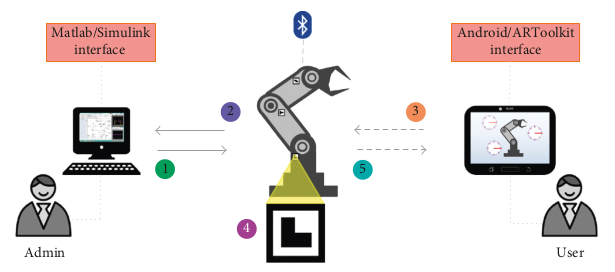
\includegraphics[width=0.98\textwidth]{Figs/SistemaAR_Maestria1}
     \end{center}
     \begin{enumerate}
     \setcounter{enumi}{4}
     \item The mobile application receives the degree of each articulation and displays them using a virtual degree protractor.
     
     \note[item]{\scriptsize  For this step, the mobile app uses the coordinates of each articulation obtained from the image obtained from the device's back camera. }
     \end{enumerate}
     
     \end{column}
     \end{columns}
\end{block}
\end{frame} 

\begin{frame}{\citetitle{MarcoNuno_Revista_2018_08_00} (3)}
\begin{block}{Results} 
\begin{columns}
\begin{column}{0.5\textwidth}
Hardware Tools:
\begin{itemize}
\item An Arduino ONE device
\item A HC-05 Bluetooth module
\item A Homemade robotic arm
\item A mobile device with back camera and Bluetooth
adapter.
\note[item]{\scriptsize In the top, we can see the integration of the components of the proposed system: (a) robotic arm and desktop application for monitoring; (b) mobile application and its interaction with the robotic arm. }
\note[item]{\scriptsize In the bottom, we can see the Robotic arm AR interface: initial position (left); real-time angle measurements (right). }
\end{itemize}
The Mobile app was tested on five different smartphones and tablet devices
\end{column}
\begin{column}{0.5\textwidth}
\begin{center}
     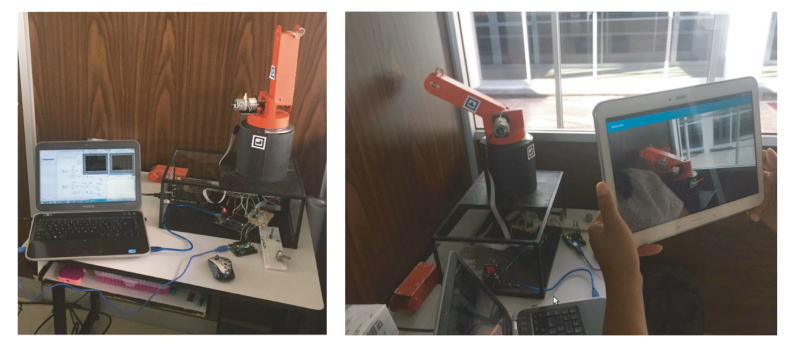
\includegraphics[width=0.99\textwidth]{Figs/SistemaAR_Maestria3}
     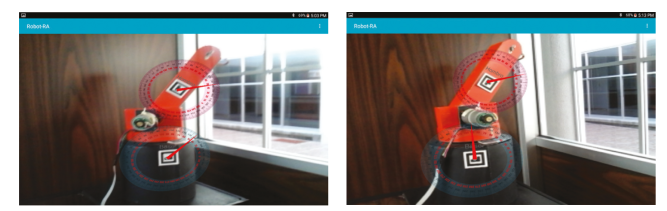
\includegraphics[width=0.99\textwidth]{Figs/SistemaAR_Maestria4}
     \end{center}
\end{column}
\end{columns}


\end{block} 
\end{frame}

%In this work, basic techniques combining augmented reality have been applied for the visualization of the articulation arm angles
% The proposed platform allows capturing the student’s attention, facilitating the understanding of complex robotics and kinematics concepts
% The implementation of a smartphone-based application will allow a large number of students to access to this type of educational resources, improving their performance and their understanding of key concepts of robotics and kinematics.

